%%% ======= Beamer ======
\documentclass[usenames,dvipsnames,t]{beamer}
% \documentclass[usenames,dvipsnames, handout]{beamer}
\beamertemplatenavigationsymbolsempty % remove toolbar at the bottom of slides
\usepackage{appendixnumberbeamer} % for appendix
\usetheme{Madrid}
\usecolortheme{default}
\useinnertheme{circles}

\usepackage{fontawesome}
\usepackage{colortbl}  % For \cellcolor in tables


% Define commands for social media icons with links
\newcommand{\linkedin}{\href{https://www.linkedin.com/in/ThibeauWouters}{\textcolor{black}{\faLinkedin}}}
\newcommand{\github}{\href{https://github.com/ThibeauWouters}{\textcolor{black}{\faGithub}}}
\newcommand{\myemail}{\href{mailto:t.r.i.wouters@uu.nl}{\textcolor{black}{\faEnvelope}}}

\newcommand{\ghlink}[1]{\href{https://github.com/#1}{\textcolor{black}{\faGithub}}}

\definecolor{customblue}{HTML}{7db8dc}
\newcommand{\thetaeos}{\boldsymbol{\theta}_{\rm{EOS}}}
\newcommand{\boldtheta}{\boldsymbol{\theta}}

\setbeamercolor{author in head/foot}{bg=blue!10, fg=blue}
\setbeamercolor{title in head/foot}{bg=blue!10, fg=blue}
\setbeamercolor{date in head/foot}{bg=blue!10, fg=blue}

\makeatletter
\setbeamertemplate{footline}{
  \leavevmode%
  \hbox{%
  \begin{beamercolorbox}[wd=.333333\paperwidth,ht=2.25ex,dp=1ex,center]{author in head/foot}%
    \usebeamerfont{author in head/foot}\insertshortauthor\expandafter\ifblank\expandafter{\beamer@shortinstitute}{}{~~(\insertshortinstitute)}
  \end{beamercolorbox}%
  \begin{beamercolorbox}[wd=.333333\paperwidth,ht=2.25ex,dp=1ex,center]{title in head/foot}%
    \usebeamerfont{title in head/foot}\insertshorttitle
  \end{beamercolorbox}%
  \begin{beamercolorbox}[wd=.333333\paperwidth,ht=2.25ex,dp=1ex,right]{date in head/foot}%
    \usebeamerfont{date in head/foot}\insertshortdate{}\hspace*{2em}
    \insertframenumber{}%
%     / \inserttotalframenumber
    \hspace*{2ex}
  \end{beamercolorbox}}%
  \vskip0pt%
}
\makeatother

% Show the TOC at the beginning
\AtBeginSection[]{
  \addtocounter{framenumber}{-1}
  \begin{frame}[plain]
      \frametitle{Contents}
      \tableofcontents[currentsection,subsectionstyle=shaded/shaded/hide]
  \end{frame}
}

% Show TOC at beginning of each subsection
\AtBeginSubsection[]{
  \addtocounter{framenumber}{-1}
  \begin{frame}[plain]
      \frametitle{Contents}
      \tableofcontents[currentsection, currentsubsection, subsectionstyle=show/shaded/hide]
  \end{frame}
}


\colorlet{beamer@blendedblue}{blue!70} % change color theme

\usepackage[style=numeric-comp,sorting=none,backend=biber]{biblatex}%<- specify style
\addbibresource{references.bib}%<- specify bib file

\usepackage[inkscapearea=page]{svg}
\usepackage{adjustbox}


% For appendix
\newcommand{\backupbegin}{
   \newcounter{framenumberappendix}
   \setcounter{framenumberappendix}{\value{framenumber}}
}
\newcommand{\backupend}{
   \addtocounter{framenumberappendix}{-\value{framenumber}}
   \addtocounter{framenumber}{\value{framenumberappendix}}
}

\setbeamertemplate{bibliography item}{\insertbiblabel} % improved references



% Other preamble stuff:
\usepackage{preamble}

% For figures
\usepackage{import}
\usepackage{xifthen}
\usepackage{pdfpages}
\usepackage{transparent}
\usepackage{mdframed}
\usepackage{subcaption}

\setbeamertemplate{caption}[numbered]

\usepackage{multirow}


% --- Inkscape figures:
\newcommand{\incfig}[2][0.75\textwidth]{%
    \def\svgwidth{\columnwidth}
    \resizebox{#1}{!}{\import{Inkscape/}{#2.pdf_tex}}
}

% --- Height of frame
\newlength{\myheight}
\setlength{\myheight}{7cm}

\newlength\myheightfigureintext
\newlength\mydepthfigureintext
\settototalheight\myheightfigureintext{Xygp}
\settodepth\mydepthfigureintext{Xygp}
\setlength\fboxsep{0pt}

\usepackage{tikz}
\usepackage[absolute,overlay]{textpos} % for precise positioning

\usepackage{ifthen}


%------------------------------------------------------------
%This block of code defines the information to appear in the
%Title page
\title[EOS systematics] %optional
{Equation of state inference systematics in the ET era with \texttt{jester}}

\author[Thibeau Wouters]{Thibeau Wouters \\ \vspace{2mm} \href{mailto:t.r.i.wouters@uu.nl}{t.r.i.wouters@uu.nl} \newline \github \quad \linkedin \quad \myemail}

\date{ET div. 6 25/03/2026}

%End of title page configuration block
%------------------------------------------------------------



%------------------------------------------------------------
%The next block of commands puts the table of contents at the
%beginning of each section and highlights the current section:

%------------------------------------------------------------


\begin{document}

{
\usebackgroundtemplate{\transparent{0.5}{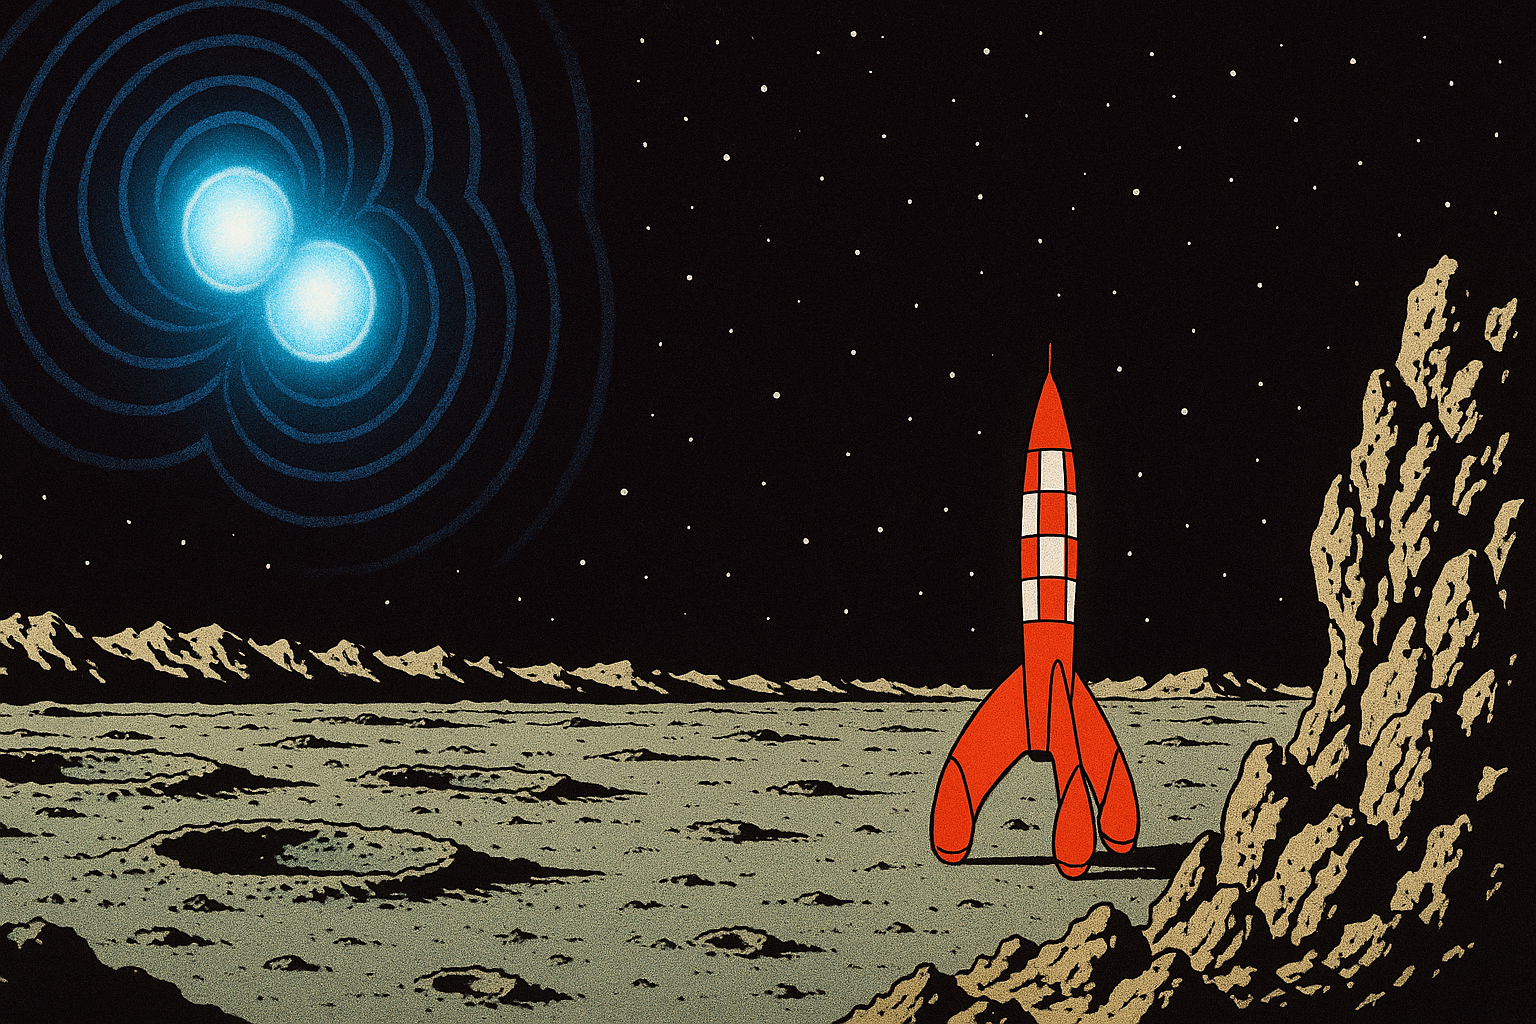
\includegraphics[width=\paperwidth,height=\paperheight]{Figures/tintin_BNS_2.png}}}

\begin{frame}[plain, noframenumbering]

  \begin{tikzpicture}[remember picture,overlay]
    \node[fill=customblue, fill opacity=0.75, text opacity=1, rounded corners=10pt, inner sep=15pt] at (current page.center) {
      \begin{minipage}{0.8\textwidth}
        \centering
        Equation of state inference systematics in the ET era \\[2.0ex]
        Thibeau Wouters \\[0.5ex]
        \github \quad \linkedin \quad \myemail
      \end{minipage}
    };
  \end{tikzpicture}

  \vspace{7cm}

  \begin{columns}
  \column{0.35\textwidth}
  \begin{figure}
    \centering
    \vspace{1.5mm}
    
\includegraphics[width=0.75\linewidth]{Figures/utrecht-university.png}
  \end{figure}
  \column{0.35\textwidth}
  \begin{figure}
    \centering
    
\includegraphics[width=0.75\linewidth]{Figures/Nikhef_logo-transparent.png}
  \end{figure}
\end{columns}

  \end{frame}
}


\begin{frame}[noframenumbering]
\frametitle{Table of Contents}
\tableofcontents[hideallsubsections]
\end{frame}

\section{Introduction}


\begin{frame}{Motivation}
  \def\x{4mm}
  \def\y{2mm}

  ET div. 6 roadmap on EOS inference:
  \begin{itemize}
    \item ``Studies to quantify the main sources of systematics in EoS inference.''
  \end{itemize}

  \vspace{\x}

  CE STM:
  \begin{itemize}
    \item ``The inference of the EOS from the $M-\Lambda$ data will allow us to make (model-dependent) statements on properties of nuclear matter, like the symmetry energy and its slope at saturation density''

    \vspace{\y}

    \item ``we will be able to make statements about how strongly a given detector con-,guration can constrain deviations from nuclear physics''
  \end{itemize}

  \vspace{\x}

  \begin{tcolorbox}[colback=blue!5!white,colframe=blue!75!black,title=Motivation]
      How will we do this in practice?
  \end{tcolorbox}

\end{frame}

\begin{frame}{Motivation}
  \def\x{4mm}
  \def\y{1mm}

  Goal:
  \begin{itemize}
    \item Bayesian inference of EOS parametrization with multimessenger data $d$: using stochastic samplers
    \begin{equation*}
      P(\thetaeos | d, \mathcal{H}) = \frac{P(d | \thetaeos, \mathcal{H}) P(\thetaeos | \mathcal{H})}{P(d | \mathcal{H})} \, .
    \end{equation*}

    \vspace{\y}

    \item Understand systematics in this inference problem
  \end{itemize}

  \pause
  \vspace{\x}

  Challenges:
  \begin{itemize}
    \item Direct EOS sampling: TOV equations are costly

    \vspace{\y}
    
    \item Multiple inferences (priors, constraints, models, samplers,...) 
    
    \vspace{\y}

    \item Handle many \& loud events in 3G
  \end{itemize}

  \pause
  \vspace{1mm}

  \begin{tcolorbox}[colback=blue!5!white,colframe=blue!75!black,title=Need]
      Scalable, flexible inference framework for multimessenger EOS data
  \end{tcolorbox}

\end{frame}


\begin{frame}{\texttt{jester}: JAX-accelerated EOS inference}
  \def\x{5mm}
  \def\y{1mm}

  \vspace{-4mm}

  \begin{columns}[t]
    \column{0.80\textwidth}
    \begin{itemize}
      \item Hierarchical EOS inference in JAX~\cite{Wouters:2025zju}
      \item GPU-accelerated TOV solvers and samplers
      \item \ghlink{nuclear-multimessenger-astronomy/jester}~\texttt{nuclear-multimessenger-astronomy/jester}
    \end{itemize}

    \column{0.20\textwidth}
    \begin{figure}
      \centering
      
\includegraphics[scale=0.05]{Figures/JESTER_logo.png}
    \end{figure}
  \end{columns}

  \vspace{\x}
  \pause

  Currently available:
  \begin{itemize}
    \vspace{\y}

    \item EOS models:
    \begin{itemize}
      \item Metamodel+speed-of-sound (MM+CSE)
      \item Spectral expansion
    \end{itemize}

    \vspace{\y}
    
    \item Samplers:
    \begin{itemize}
      \item \textsc{flowMC} % TODO: citation
      \item Nested sampling (NS)
      \item Sequential Monte Carlo (SMC)
    \end{itemize}

    \vspace{\y}

    \item Constraints: GW posterior ($m_i$, $\Lambda_i$), nuclear physics,\dots
  \end{itemize}
\end{frame}


\section{Results}

\begin{frame}{EOS inference systematics in ET}
  \def\x{6mm}
  \def\y{2mm}

  Simulated study for Einstein Telescope (ET):
  \begin{itemize}
    \vspace{\y}
    \item 100 loudest BNS events from 1 year (CoBa catalogue~\cite{Branchesi:2023mws})
    
    \vspace{\y}
    
    \item Injection EOS from Ref.~\cite{Koehn:2024set}: MM+CSE
    
    \vspace{\y}
    
    \item GW parameter estimation
    \begin{itemize}
      \item \texttt{IMRPhenomXP\_NRTidalv3}, $f_{\rm{min}} = 5$ Hz
      \item Relative binning
      \item \textsc{bilby}
      \item Ran by Fabian Gittins
    \end{itemize}

    \vspace{\y}

    \item \red{Preliminary results in this talk!}

  \end{itemize}
\end{frame}

\begin{frame}{EOS inference systematics in ET: Results}
  \def\x{7mm}
  \def\y{2mm}

  \vspace{\x}

  \only<1>{
    \begin{figure}
    
\includegraphics[width=0.90\textwidth]{ET_ET_lambda14_comparison.pdf}
    \end{figure}
  }

  \only<2>{
    \begin{figure}
    
\includegraphics[width=0.90\textwidth]{ET_ET_r14_comparison.pdf}
    \end{figure}
  }
  
  \only<3>{
    \vspace{-3mm}
    \begin{figure}
    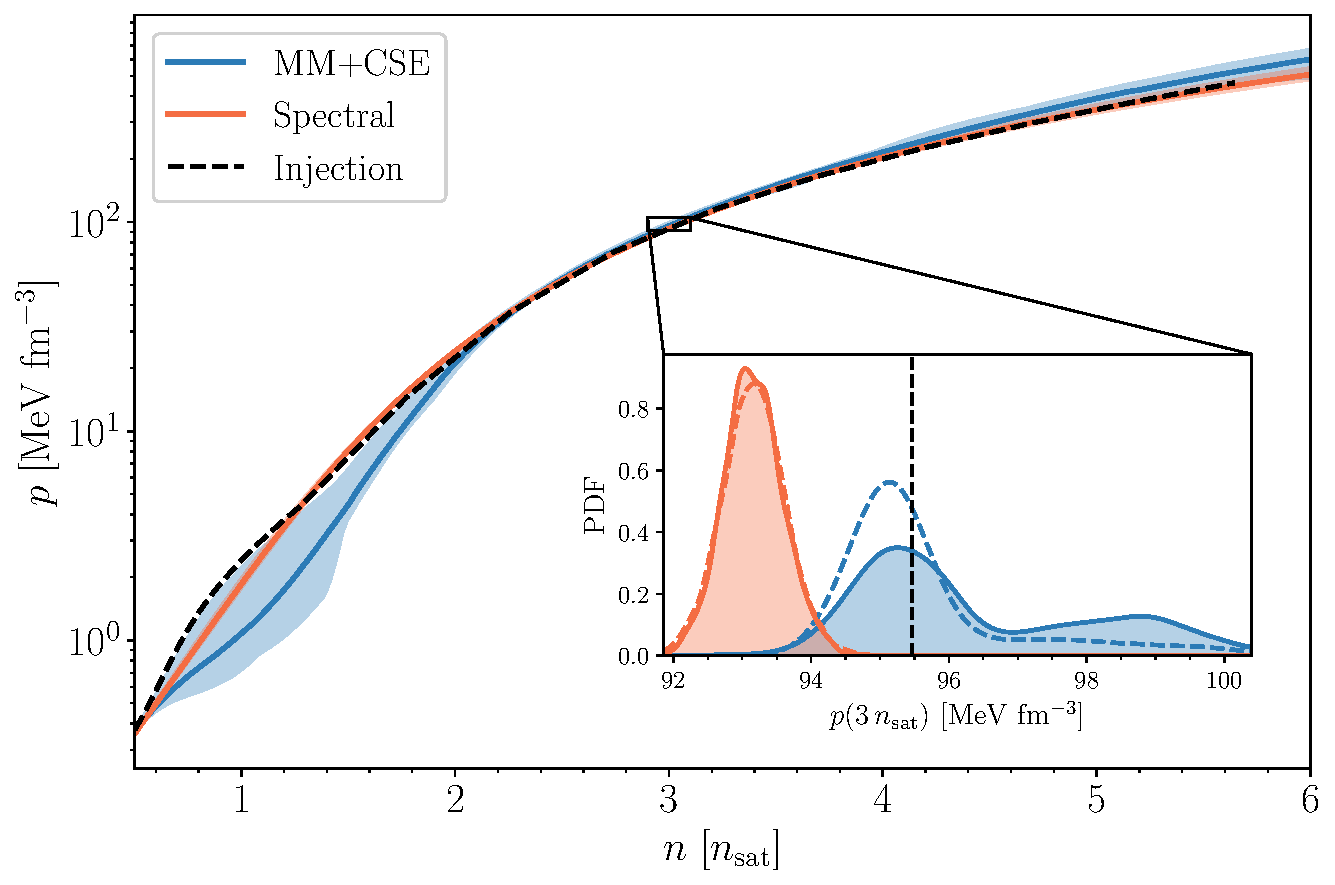
\includegraphics[width=0.90\textwidth]{Figures/ET_pressure_density_inset.pdf}
    \end{figure}
  }
  
  \only<4>{
    \vspace{-10mm}
    \begin{figure}
    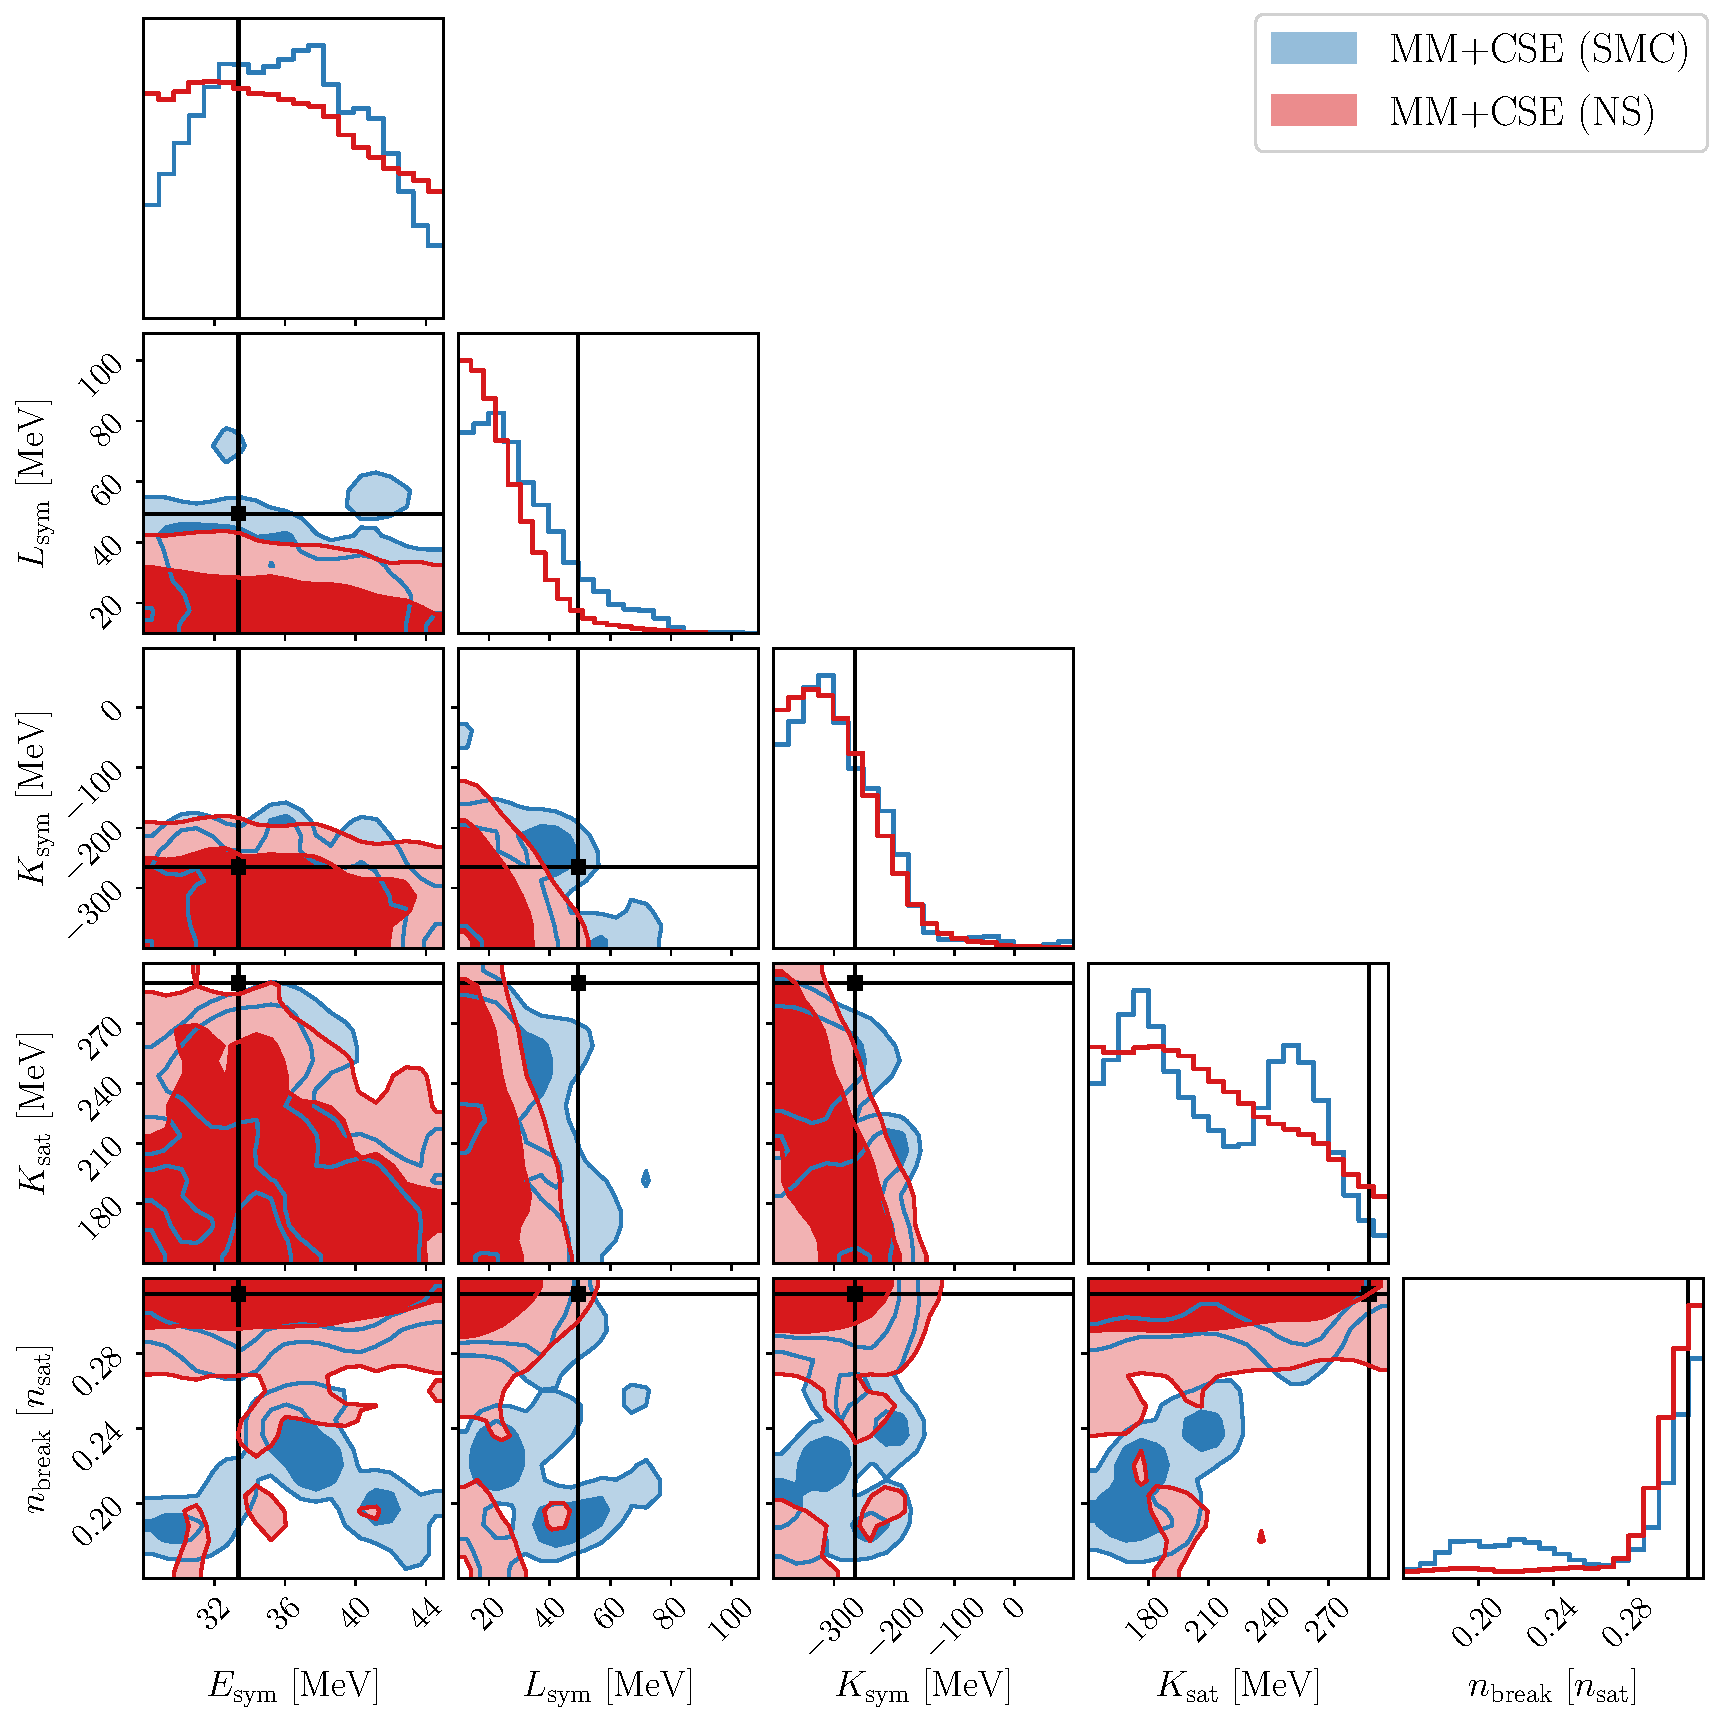
\includegraphics[width=0.675\textwidth]{Figures/ET_cornerplot_nep_E_sym_L_sym_K_sym_K_sat_nbreak.pdf}
    \end{figure}
  }

\end{frame}

\begin{frame}{EOS inference systematics in ET: Results}
  \def\x{3mm}
  \def\y{2mm}

  % \vspace{-4mm}
  %   \begin{table}[h]
  %     \centering
  %     \renewcommand{\arraystretch}{1.4}
\begin{tabular}{p{4.5cm}cc}
    \hline
    EOS model & Sequential Monte Carlo & Nested Sampling \\
    \hline
    Metamodel\newline + speed-of-sound & $12.51^{+0.31}_{-0.10}$ & $12.45^{+0.29}_{-0.07}$ \\
    Spectral decomposition & $12.48^{+0.04}_{-0.03}$ & $12.48^{+0.04}_{-0.02}$ \\
    \hline
\end{tabular}

  %     \caption{$R_{1.4}$ [km] at 90\% credibility.} 
  %   \end{table}

  Inference is scalable: ideal to investigate systematics in EOS inference 

  \vspace{\x}

  \begin{table}[h]
    \centering
    \renewcommand{\arraystretch}{1.4}
\begin{tabular}{p{4.5cm}cc}
    \hline
    EOS model & Sequential Monte Carlo & Nested Sampling \\
    \hline
    Metamodel\newline + speed-of-sound & 1h 24m & 13h 07m \\
    Spectral decomposition & 20m 10s & 1h 11m \\
    \hline
\end{tabular}

    \caption{Sampling time on 1 NVIDIA H100 GPU.}
  \end{table}
\end{frame}

\section{Outlook \& Conclusion}


% \begin{frame}{Looking ahead}
%   \def\x{3mm}
%   \def\y{1mm}

%   Future extensions of \texttt{jester}:
%   \begin{itemize}
%     \vspace{\y}
%     \item More TOV solvers
%     \begin{itemize}
%       \item Pressure anisotropy~\cite{Pang:2025fes} \small (Peter T. H. Pang) \normalsize
%       \item Non-GR, e.g., scalar-tensor gravity~\cite{Brown:2024joy, Creci:2024wfu} \small (Dio Danarianto, Alex Brown) \normalsize
%     \end{itemize}

%     \vspace{\y}
    
%     \item Improved EOS physics
%     \begin{itemize}
%       \item Composition, temperature (Guilherme Grams)
%     \end{itemize}

%     \vspace{\y}
    
%     \item More neutron star physics
%     \begin{itemize}
%       \item Oscillation modes, phase transitions, postmerger,...
%     \end{itemize}
    
%     \vspace{\y}
    
%     \item More EOS parametrizations, constraints,...
%   \end{itemize}

%   \vspace{\x}

%   \begin{tcolorbox}[colback=blue!5!white,colframe=blue!75!black,title=Input welcome!]
%       What would you like to see in \texttt{jester}?
%   \end{tcolorbox}

% \end{frame}

\begin{frame}{Conclusion}
  \def\x{4mm}

  \begin{itemize}
    \item \texttt{jester}: GPU-accelerated EOS inference

    \vspace{\x}

    \item Scalable inference for multimessenger data to enable projection studies to understand systematics

    \vspace{\x}

    \item For 100 loud BNSs in ET:
    \begin{itemize}
      \item Agreement on $\Lambda_{1.4}$
      \item Differences among EOS parametrizations
      \item Samplers consistent
    \end{itemize}

    \vspace{\x}

    \item Going forward: what to investigate for ET div. 6 roadmap?
  \end{itemize}

\end{frame}

{
\usebackgroundtemplate{\transparent{0.5}{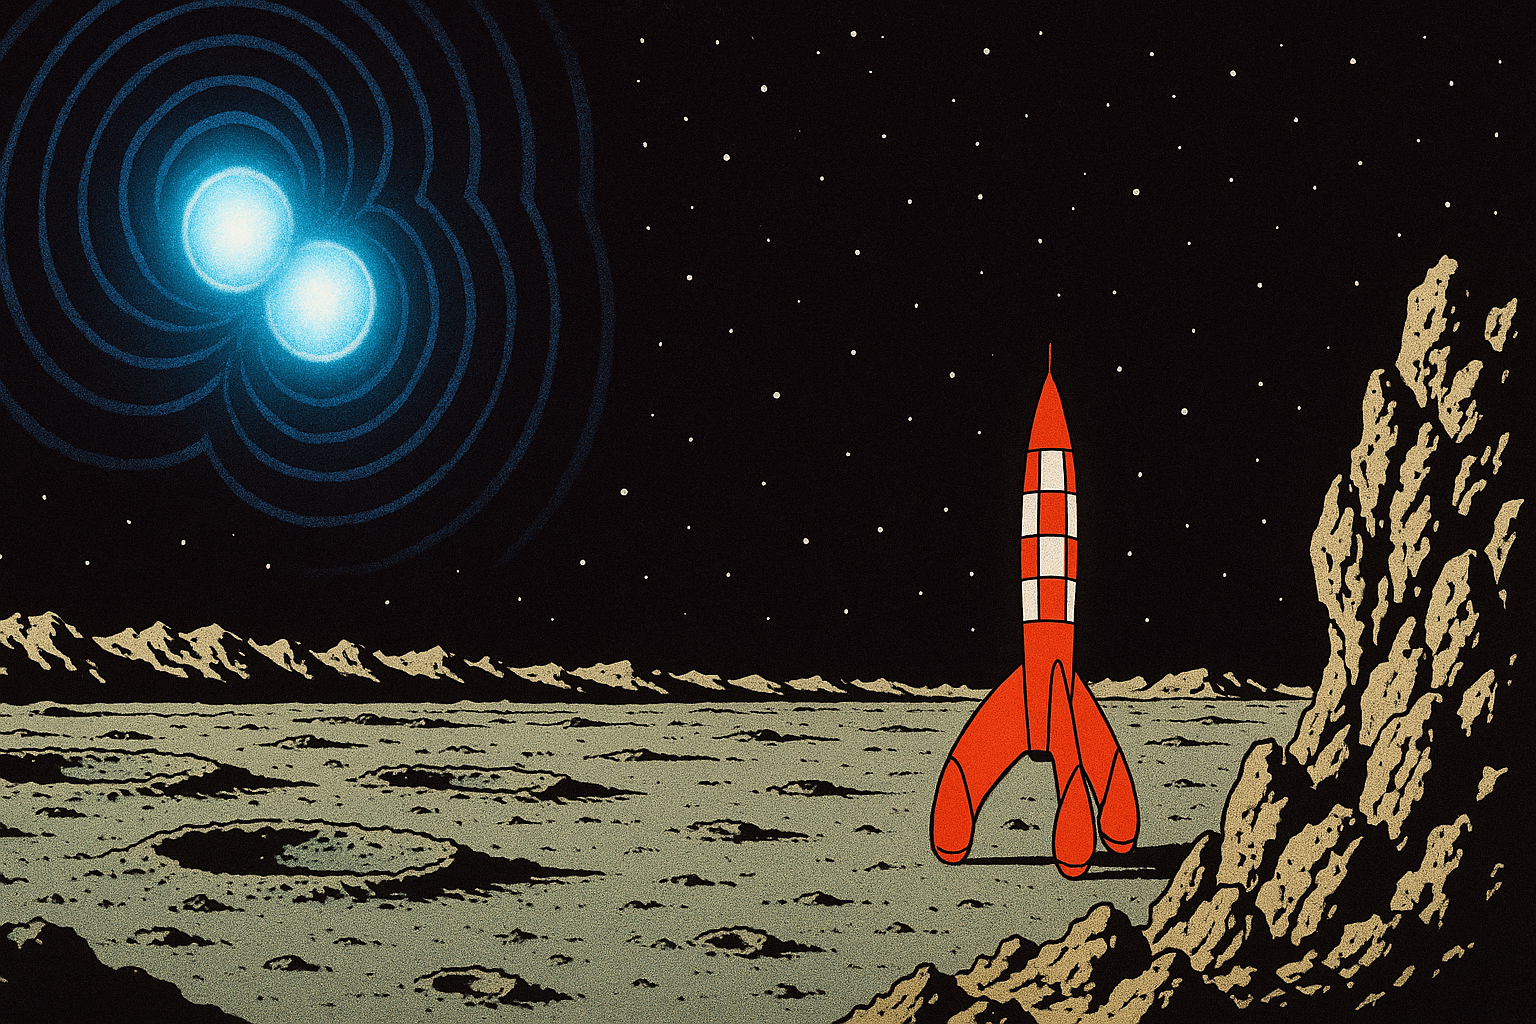
\includegraphics[width=\paperwidth,height=\paperheight]{Figures/tintin_BNS_2.png}}}

\begin{frame}[plain, noframenumbering]

  \begin{tikzpicture}[remember picture,overlay]
    \node[fill=customblue, fill opacity=0.75, text opacity=1, rounded corners=10pt, inner sep=15pt] at ([yshift=2cm]current page.center) {
      \begin{minipage}{0.8\textwidth}
        \centering
        \textbf{Thanks for listening!}
      \end{minipage}
    };
  \end{tikzpicture}

  \end{frame}
}

\begin{frame}[allowframebreaks]{References}
  \printbibliography
\end{frame}

\appendix

\begin{frame}{Sampler systematics: GW170817}
  \def\x{4mm}
  \def\y{1mm}

  Analyzing GW170817 with different EOS and samplers:

  \vspace{-4mm}
  % \vspace{\x}

  %% With radio 
  % \only<1>{
    \begin{table}[h]
      \centering
      \renewcommand{\arraystretch}{1.4}
\begin{tabular}{p{4.5cm}cc}
    \hline
    EOS model & Sequential Monte Carlo & Nested Sampling \\
    \hline
    Metamodel\newline + speed-of-sound & $12.60^{+1.04}_{-1.42}$ & $12.46^{+1.15}_{-1.38}$ \\
    Spectral decomposition & $12.49^{+1.01}_{-1.33}$ & $12.40^{+1.03}_{-1.34}$ \\
    \hline
\end{tabular}

      \caption{$R_{1.4}$ [km] at 90\% credibility.}
    \end{table}
  % }

  % \pause
  \vspace{-2mm}
  
  % \only<2>{
    \begin{table}[h]
      \centering
      \renewcommand{\arraystretch}{1.4}
\begin{tabular}{p{4.5cm}cc}
    \hline
    EOS model & Sequential Monte Carlo & Nested Sampling \\
    \hline
    Metamodel\newline + speed-of-sound & 5m 38s & 32m 18s \\
    Spectral decomposition & 2m 57s & 7m 48s \\
    \hline
\end{tabular}

      \caption{Sampling time on 1 NVIDIA H100 GPU.}
    \end{table}
  % }
\end{frame}

\begin{frame}{$\Lambda_{1.4}$ for GW170817 inference}

  \begin{figure}
    \centering
    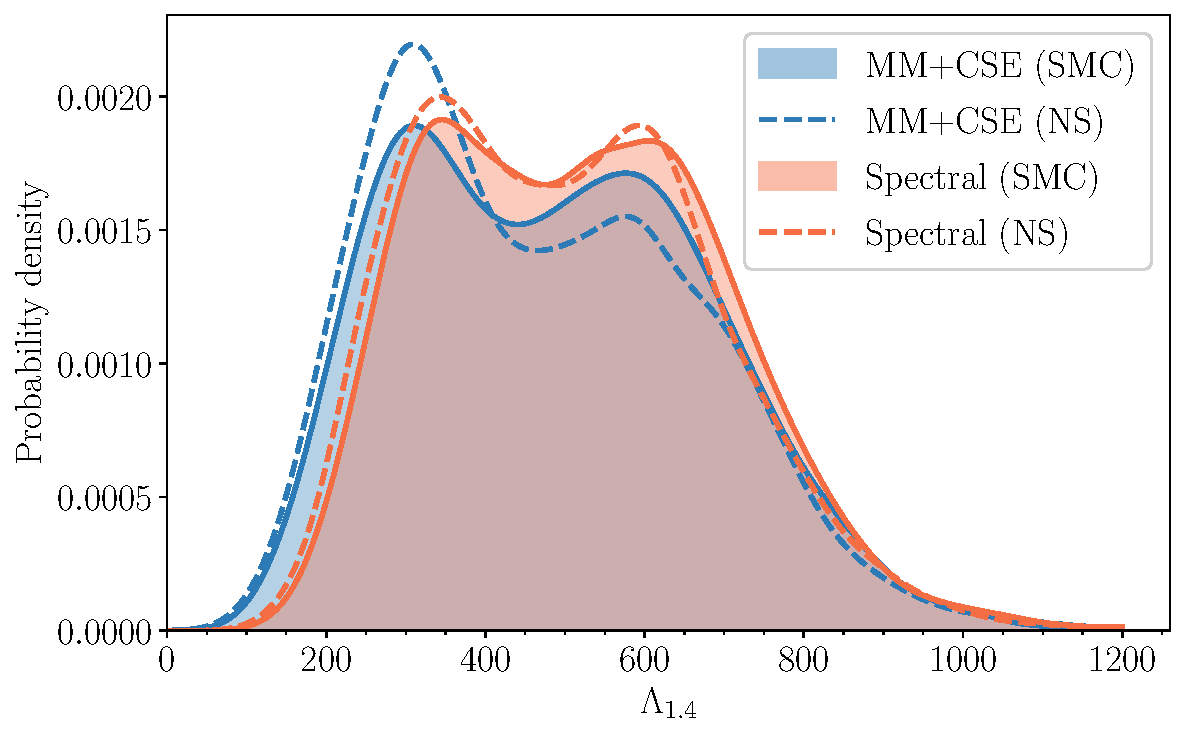
\includegraphics[width=0.90\textwidth]{SS_lambda14_comparison.pdf}
  \end{figure}
  
\end{frame}

\begin{frame}{$R_{1.4}$ for GW170817 inference}

  \begin{figure}
    \centering
    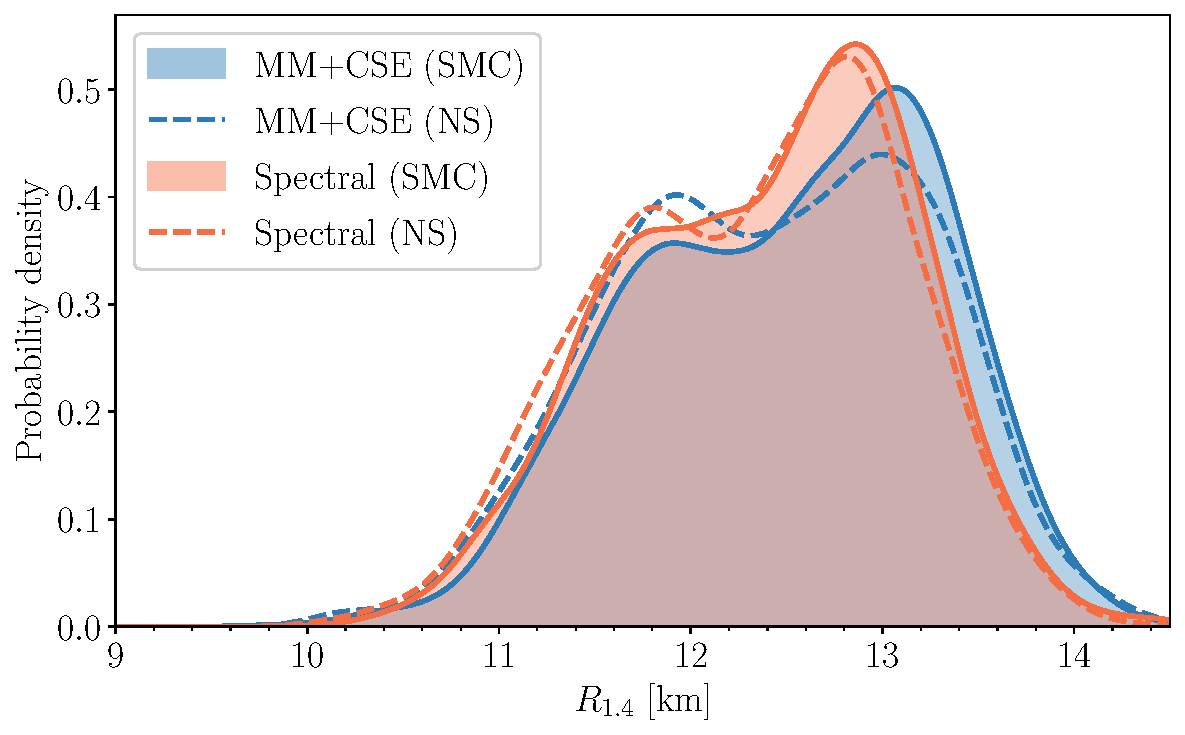
\includegraphics[width=0.90\textwidth]{SS_r14_comparison.pdf}
  \end{figure}
  
\end{frame}


\end{document}
